\chapter{Testing lepton flavour universality with $R_H$}
\label{sec:RKst_theory}

Lepton Favour Universality (LFU) is the equality of the weak coupling constants for all leptons.
%and can be broken in NP scenarios. 
FCNCs processes, forbidden in the SM at tree level and happening
only at loop level, are an ideal laboratory for studying LFU as NP in the loops could break the flavour symmetry.
 
In this work, decays of $b \rightarrow s\mumu (\ee)$ type, are considered to test LFU
between electrons and muons using penguin decays.
In particular, \Bz meson semileptonical decays to $\Bz\to\Kstarz\ll$ are considered.
Figure~\ref{fig:RKpenguins} shows the possible Feynman diagrams 
producing such decays while Fig.~\ref{fig:NPpenguins} illustrates how the Feynman 
diagrams of these processes may include new particles. 
A series of recent LHCb measurements~\cite{TomRDreview}
points to a tension with SM predictions, which make these processes very interesting
to better understand the nature of the discrepancy.
%
\begin{figure}[h]
\centering 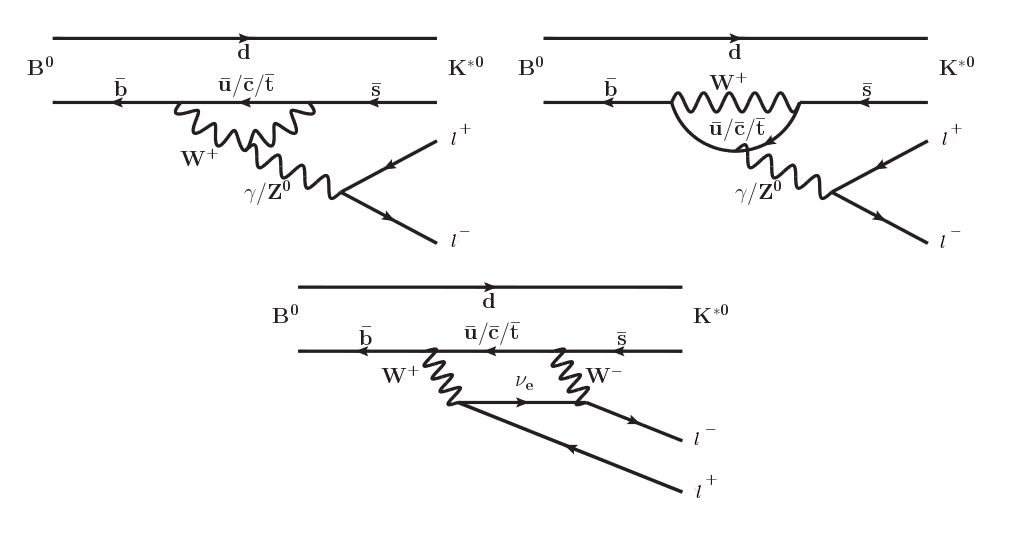
\includegraphics[width=0.8\textwidth]{RKst/figs/penguins3.png}
\caption{Loop diagrams of the $\Bz \to K^{(*0)}\ll$ process.}
\label{fig:RKpenguins}
\end{figure}

In order to exploit the sensitivity of loop diagrams, in 2004 Hiller and Kruger proposed the measurement 
of the $R_H$ ratio \cite{Hiller:2003js}, defined in Eq.~\ref{eqRX}, where $H$ can be an inclusive state containing 
an $s$ quark ($X_s$) or an s-quark resonance like $K$ or $\Kstarz$.
\begin{equation}
\label{eqRX}
R_{H} = \frac{\int_{4m_{\mu}^2}^{m_b} \frac{ d\BR(\Bd \to H \mumu) }{d\qsq}}{ \int_{4m_{\mu}^2}^{m_b}\frac{ d\BR(\Bz \to H\epem) }{d\qsq}} d\qsq
\end{equation}
In this quantity the decay width is integrated over the squared dilepton invariant mass, \qsq, from 
$\qsq_{min} = 4m_{\mu}^2$, which is the threshold for the $\mu\mu$ process, up to \mbox{$\qsq_{max} = m_b^2$.} 

%The notation $\BR(X \rightarrow ~final ~state)$ denotes the fraction of $X$ particles which decays in the 
%given final state, this is called ``branching ratio". For example $\BR(\Bz\to\Kstar\mumu)$ is the
%fraction of \Bz particles which decays into $\Kstar\mumu$ with respect to all allowed \Bz decays.

The advantage of using ratios of branching fractions as observables is that, in the theoretical prediction, hadronic 
uncertainties cancel out. Furthermore, experimentally, some of the systematic uncertainties on the ratios are reduced
giving a better measurement. For example, what is measured is the number of $\mu\mu$ and $ee$ decays 
which happen in a certain period of time. Then, the luminosity, $\mathcal{L}$, is used to obtain a
cross section, $\sigma$, using $R = \mathcal{L}\sigma$, where $R$ is the rate at which the decays happen. 
The luminosity measurement is usually a source of systematic uncertainty, however it appears on both
sides of the ratio and therefore cancels out.

\begin{figure}[h]
\centering 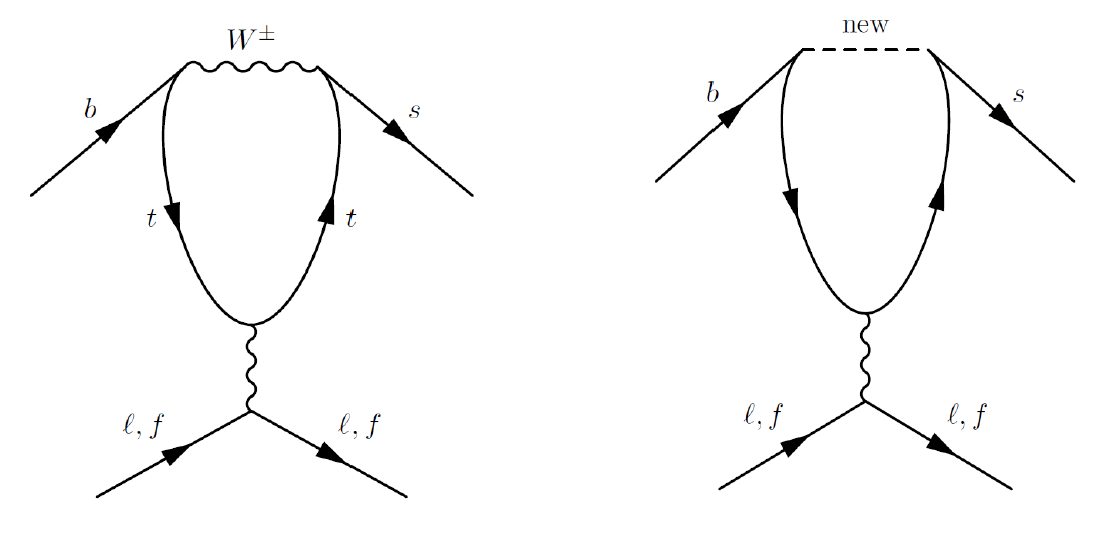
\includegraphics[width=0.8\textwidth]{RKst/figs/penguins.png}
\caption{Example of penguin diagrams, on the left involving SM particles and on the right 
involving new possible particles.}
\label{fig:NPpenguins}
\end{figure}

Since the SM does not distinguish between lepton flavours, the predicted value of the ratio 
is $R_H = 1$, under the assumption of massless leptons. Taking into account effects of order 
$m_\mu^2 / m_b^2$ Hiller and Kruger calculate that in the SM and in the full \qsq range~\cite{Hiller:2003js}:
%
\begin{align}
R_{X_s} = 0.987 \pm 0.006 \\
R_K = 1.0000 \pm 0.0001 \\
R_{\Kstarz} = 0.991 \pm 0.002 \\
\end{align}
%
\noindent
under the assumptions that:
%
\begin{itemize}
\item right-handed currents are negligible;
\item (pseudo-)scalar couplings are proportional to the lepton mass;
\item there are no CP-violating phases beyond the SM.
\end{itemize}

The measurement of the $R_H$ ratios is of particular interest after the recent
measurement of the branching ratio of the $\Bs\to\mumu$ decay~\cite{CMS:2014xfa}, 
where no evidence of NP was found. In fact the quantities $(R_H - 1)$ and
$\BR(\Bs \to \mumu)$ remain proportional with
%
\begin{equation}
\frac{R_H - 1}{\BR(\Bs \to \mumu)} \sim 2 \cdot 10^{-5}
\end{equation}
%
A joint measurement of this two quantities can give much information and constrain MFV models.
If $R_H = 1$ and $\BR(\Bs \to \mumu)$ is close to the SM prediction as it is measured to be
this will allow to put strong constraints on extensions of the SM.
If instead $R_H > 1$ and the equation above is not verified, this would mean that one of the
assumptions listed above are not verified, which can happen is some extensions of the SM
as Super-Symmetric models with broken R-parity.
A series of recent LHCb measurements~\cite{TomRDreview} shows tensions with
SM predictions, which makes it interesting to further investigate these processes.

\subsection{Combining ratios}

The full power of the $R_H$ ratios in understanding new physics scenarios comes from
their combinations.  In Ref.~\cite{Hiller:2014ula} Hiller and Schmaltz propose the measurement 
of the double ratios, $X_H = R_H / R_K$, which not only can test LFU but also allow
to disentangle the kind of new physics that lies behind. These ratios are in fact sensitive
to FCNCs of right-handed currents. Furthermore, in Ref.~\cite{Hiller:2014ula} the study is extended
to \Bs decays such as $\Bs\to\phi\ll$ or $\Bs\to\eta\ll$.

Parity and Lorentz invariance require that the Wilson Coefficients with left-handed chirality ($C$)
and their right-handed counterparts ($C'$) appear in the decay amplitude of exclusive decays in
determined combinations, e.g.
\begin{equation}
\begin{array}{ll}
C+C': & K, \Kstar_{\perp}, ...  \\
C-C': & K_0(1430), \Kstar_{0,\parallel}, ...
\end{array}
\end{equation}
where the labels for the \Kstar meson represent its longitudinal (0), parallel $(\parallel)$ and
perpendicular $(\perp)$ transversity components. The $C$ contributions are universal to
all decays and therefore $X_H$ double ratios are sensitive to right-handed currents.
In fact the $R_H$ ratios can be expressed is terms of their deviation from unity as
\begin{equation}
\begin{array}{rl}
R_K \simeq 			& 1+ \Delta_+ 		\\
R_{K_0(1430)} \simeq 	& 1+ \Delta_-		\\
R_\Kstar \simeq 		& 1+ p(\Delta_- - \Delta_+) + \Delta_+
\end{array}
\end{equation}
where the $\Delta_\pm$ quantities are combinations of Wilson coefficients
described in Eq.~10 of Ref.~\cite{Hiller:2014ula} and the parameter $p$ is the polarisation of \Kstar
that in Ref.~\cite{Hiller:2014ula} is determined to be close to 1 simplifying the formula to $R_{\Kstar} \simeq 1+ \Delta_-$.
In particular one can observe the following correlations: 
\begin{itemize}
\item $R_K < 1$, as it is measured to be, and $X_{\Kstar} > 1$ points to dominant BSM contributions into $C_{LR}$ (see definition in Sec.~\ref{sec:operators});
\item a SM like $R_K \sim 1$ together with $X_{\Kstar} \neq 1$ requires BSM with $C_{LL} + C_{RL} \simeq 0$;
\item $R_K \neq 1$ and $X_{\Kstar} \simeq 1$ corresponds to new physics in $C_{LL}$.
\end{itemize}

\subsection{Experimental status}

The $R_K$ and $R_{\Kstarz}$ ratios have already been measured at the B-factories~\cite{Lees:2012tva,Wei:2009zv},
and the $R_K$ ratio has been also recently measured at LHCb~\cite{LHCb-PAPER-2014-024} in the $1 < \qsq < 6$~\gevgevcccc \qsq interval, which represents the most precise measurement to date. This measurement manifests a 2.6$\sigma$
deviation from the SM prediction. 
The current experimental status is summarised in Tab.~\ref{tab:expstatus}. By profiting of the large dataset collected during Run-I, the LHCb experiment is expected
to reduce the uncertainty on $R_{\Kstarz}$ by at least a factor of 2 with respect to the B-factories.

\begin{center}
\begin{table}[h!]
\centering
\caption{Experimental status of the $R_{K^{(*)}}$ measurements. } %by the BaBar~\cite{Lees:2012tva} and Belle~\cite{Wei:2009zv} experiment.}
\begin{tabular}{c|c|c|c}
 	& Belle 			& BaBar 		& LHCb \\
 \hline
$R_K$			& $1.06 \pm 0.48 \pm 0.05$	& $1.38^{+0.39+0.06}_{-0.41-0.07}$ & $0.745^{+0.090}_{-0.074} \pm 0.036$\\
$R_{\Kstarz}$	& $0.93 \pm 0.46 \pm 0.12$	& $0.98^{+0.30+0.08}_{-0.31-0.08}$ & ----\\
\end{tabular}
\label{tab:expstatus}
\end{table}
\end{center}


\section{Analysis strategy}

The aim of this analysis is to measure the $R_{\Kstarz}$ ratio using $pp$ collision data collected by the LHCb
detector in 2011 and 2012, corresponding to a total of 3 \invfb of integrated luminosity.
The $\Bz \to \Kstarz\mumu$ and $\Bz \to \Kstarz\epem$, ``rare channels", are
reconstructed with the $\Kstarz$ decaying into a kaon and a pion with opposite charges.

The analysis has to separate signal candidates from background candidates which have similar observed properties. 
The selection presented in Sec. \ref{sec:RKst_selection} aims to maximise the yield while minimising
the background contamination. Two types of backgrounds are identified: ``peaking background" and ``combinatorial background". 
The first comes from the mis-reconstruction of other decays or from partially reconstructed events. This type 
of background,  because its specific kinematic properties, usually peaks in some variable, such as the invariant
mass of all final particles, therefore we can remove these events by removing the peak. 
The combinatorial background  instead comes from the random combination of particles and can 
be lowered selecting events with good-quality tracks and vertices.

To further reduce systematic uncertainties the measurement is performed as a double ratio as shown in
Eq.~\ref{eq:RKst} %This exploits the charmonium decays with same final states as the considered rare ones.
where decays reaching the same final states as the rare channels via a \jpsi resonance, $\Bz\to\Kstarz(\jpsi\to\ll)$,
also referred as ``charmonium" or ``resonant" channels, are used as control samples.
These decays are distinguished from the rare channels using the invariant mass of the dilepton pair.

In Sec.~\ref{sec:RKst_efficiency} the efficiency of selecting and reconstructing each channel is extracted
and, finally, in Sec.~\ref{sec:RKst_result} the $R_{\Kstar}$ ratio defined is built as the double ratio
of rare and resonant channels:

\begin{equation}
\label{eq:RKst}
R_{\Kstarz} = 
\frac{N_{\Bz\to\Kstarz \mumu}}{N_{\Bz\to\Kstarz\jpsi\to \mumu}} 
\cdot \frac{N_{\Bz\to\Kstarz \jpsi \ee}}{N_{\Bz\to\Kstarz\ee}}
\cdot \frac{\varepsilon_{\Bz\to\Kstarz \jpsi \to \mumu}}{\varepsilon_{\Bz\to\Kstarz \mumu}} 
\cdot \frac{\varepsilon_{\Bz\to\Kstarz \ee}}{\varepsilon_{\Bz\to\Kstarz\jpsi\to \ee}}
\end{equation}

As NP is expected not to affect charmonium resonances the ratio of the \jpsi channels
is 1 and therefore $R_{\Kstarz}^{'} = R_{\Kstarz} \times R_{\jpsi} = R_{\Kstarz}$.
On the other hand using the relative efficiencies between the rare and resonant channels
allows to cancel out many effects resulting in a better control of systematic uncertainties.  

For brevity, the rare channels will also be denoted as ``$\ell\ell$", or
specifically ``$ee$'' and ``$\mu\mu$'', and the resonant channels as ``$\jpsi(\ell\ell)$'',
or ``$\jpsi(ee)$'' and ``$\jpsi(\mu\mu)$''.

\section{Choice of \qsq intervals}
\label{sec:RKst_q2_choice}

Two \qsq intervals are considered in this work: 
\begin{itemize}
\item the ``central-\qsq" region, [1.1,6.0]~\gevgevcccc;
\item the ``high-\qsq "region, above 15~\gevgevcccc.
\end{itemize}
%
The central-\qsq region is the most interesting place to look for new physics. In fact, at low \qsq, below 
1~\gevgevcccc~the photon pole dominates leaving little space for NP to be found~\cite{TomRDreview}.
The upper bound of this interval is set at 1.1~\gevgevcccc, in order entirely include the contribution
from $\phi\to\ll$ decays, that can dilute new physics effects, into the low \qsq interval.
The upper bound of the central interval is chosen to be sufficiently far away from the \jpsi radiative
tail, where predictions cannot be cleanly extracted. The 6--15~\gevgevcccc~region is characterised by the presence
of the narrow peaks of the \jpsi and \psitwos resonances. The lower bound of the high-\qsq region, where
the signal in the electron channel is still unobserved, is chosen to be sufficiently far from the \psitwos resonance.
Rare and resonant channels are selected depending on which \qsq interval they fall in (for details see Sec.~\ref{sec:RKst_selection}).


\section{Data samples and simulation}

This analysis is based on a data set corresponding to 3~\invfb of integrated
luminosity collected by the LHCb detector in 2011 and 2012.
In order to study the background properties, determine efficiencies and to train the multivariate analysis
simulated events are used. After the hard interactions are generated with Pythia8 hadronic particles
are decayed using EvtGen and, finally, propagated into the detector using Geant4 and reconstructed
with the same software used for data. Samples are generated with both 2011 and 2012, magnet up and down
 conditions and are combined in the right proportions, according to the luminosity registered on data.
The next section describes the corrections applied to the simulation to obtain a better description of data.

%distributions of key valiables were compared between data and simulation and correction 
%In Table \ref{TabMC} are reported the MC samples used
%together with the number of generated events and the branching fractions of the simulated processes

\subsection{Data-simulation corrections}
\label{sec:RKst_mc_weighting}

Since the multivariate classifier training (see Sec.~\ref{sec:RKst_mva}) and the calculation
of most of the efficiency components (see Sec.~\ref{sec:RKst_efficiency}) are obtained from
the study of simulated events it is important to verify that the simulation is a reliable
reproduction the data. In particular it is important to match data and Monte Carlo
in the kinematics of the final particles and the occupancy of the detector.
The kinematics of the decays is characterised by the transverse momentum spectrum of
the \Bz. Discrepancies in this distribution cause also the spectra of the final particles
to differ from data and affect the efficiency determination as its value often
depends on the momentum distribution of final particles.
The occupancy of the detector is correlated to the invariant mass shape of the signal because
the addition of energy clusters in the electromagnetic calorimeter,
affects the electron momenta for bremsstrahlung photons emitted before the magnet.
The hit multiplicity in the SPD detector is a proxy for the detector occupancy.

Since it is important that these quantities are well modelled, the simulation is
reweighted so that the distributions in data and simulation match for these variables.
This can be done using resonant $\decay{\Bz}{\Kstarz(\jpsi\to\ll)}$ events, for which the signal peak
is already visible in data after pre-selection (see Sec.~\ref{sec:RKst_selection}). However, the data still includes
a high level of background and distributions cannot be directly compared.
The $_s\mathcal{P}$lot technique~\cite{sPlot} is used to statistically subtract the background from
data and obtain pure signal distributions using the invariant mass as control variable.
%This method is based on an estimation
%od the signal and background densities based on a fit to a control variable where
%the two are well distinct, usually the invariant mass.
Fig.~\ref{fig:RKst_sW_mass} shows fits to the 4-body invariant mass of candidates after pre-selection.
done in order to estimate the signal density. Data and simulation are then compared 
and the ratio between the distributions is used to re-weight the Monte Carlo. The discrepancy 
in the SPD hits multiplicity is solved as a first step and then the \Bz transverse momentum 
distributions are compared between data and simulation reweighted for the SPD multiplicities only.
Distributions of \Bz transverse momentum and SPD multiplicities are reported in Fig.~\ref{fig:b0pt_nSPD_distrib}
and ratios of these distribution, which are used to re-weight the simulation, are reported in 
Fig.~\ref{fig:b0pt_nSPD_ratios}. The weights for the SPD multiplicity are calculated
separately for 2011 and 2012 events, because distributions are significantly different
in the two years. Binnings for these distributions are chosen to have approximately 
the same number of events in each bin to limit fluctuations.
Further corrections are made re-weighting simulated events for PID efficiency using the
\verb!PIDCalib! package as described in Sec.~\ref{sec:RKst_pid_eff} and, finally, 
$ee$ samples are also reweighted for L0 trigger efficiency as described in Sec.~\ref{sec:RKst_trigger_eff}.
Weights are always applied throughout unless specified.
%Finally in Fig.~\ref{fig:mc_data_comparison} distributions of other variables are compared
%between data and reweighted Monte Carlo and show that a good agreement is achieved.

 \begin{figure}[h!]
\centering
%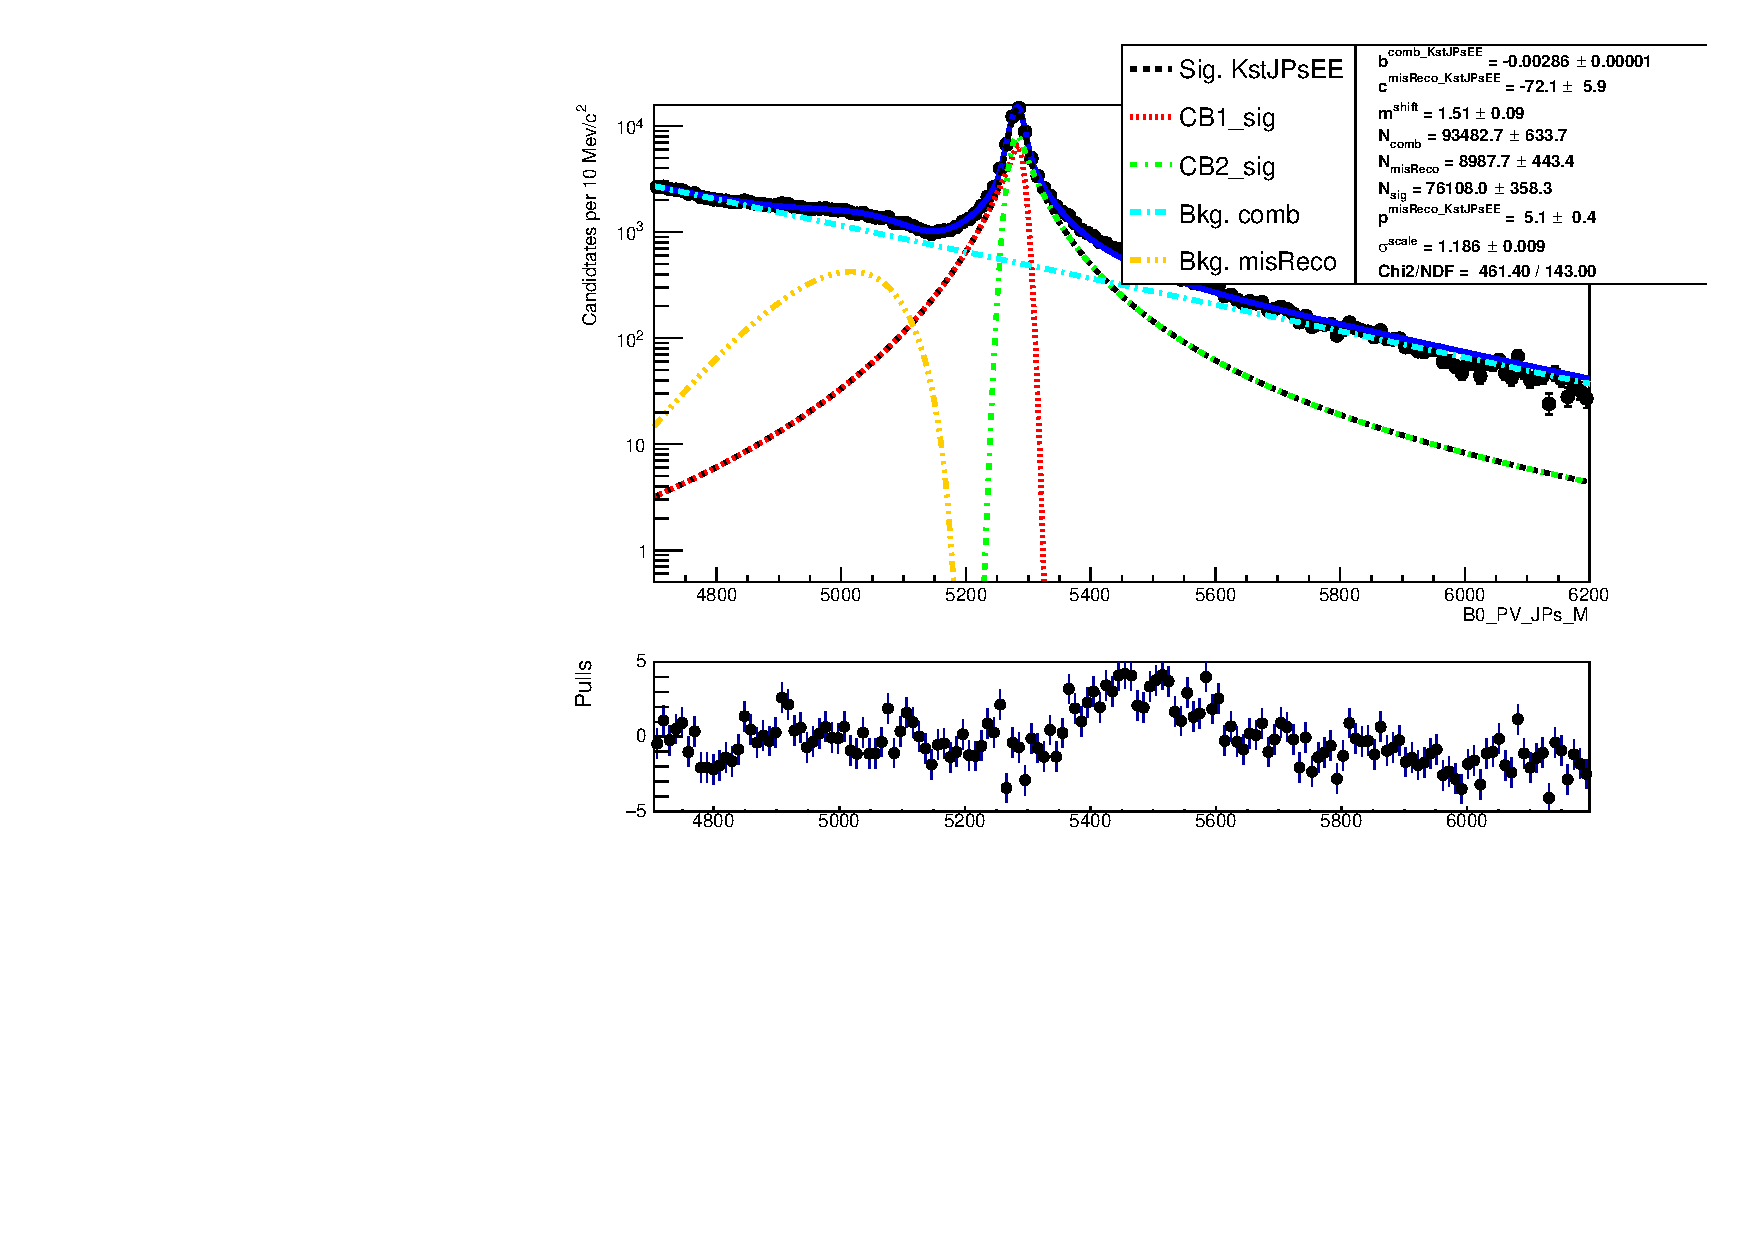
\includegraphics[width=0.48\textwidth]{RKst/figs/sW/KstJPsEE_log_fitAndRes.pdf}
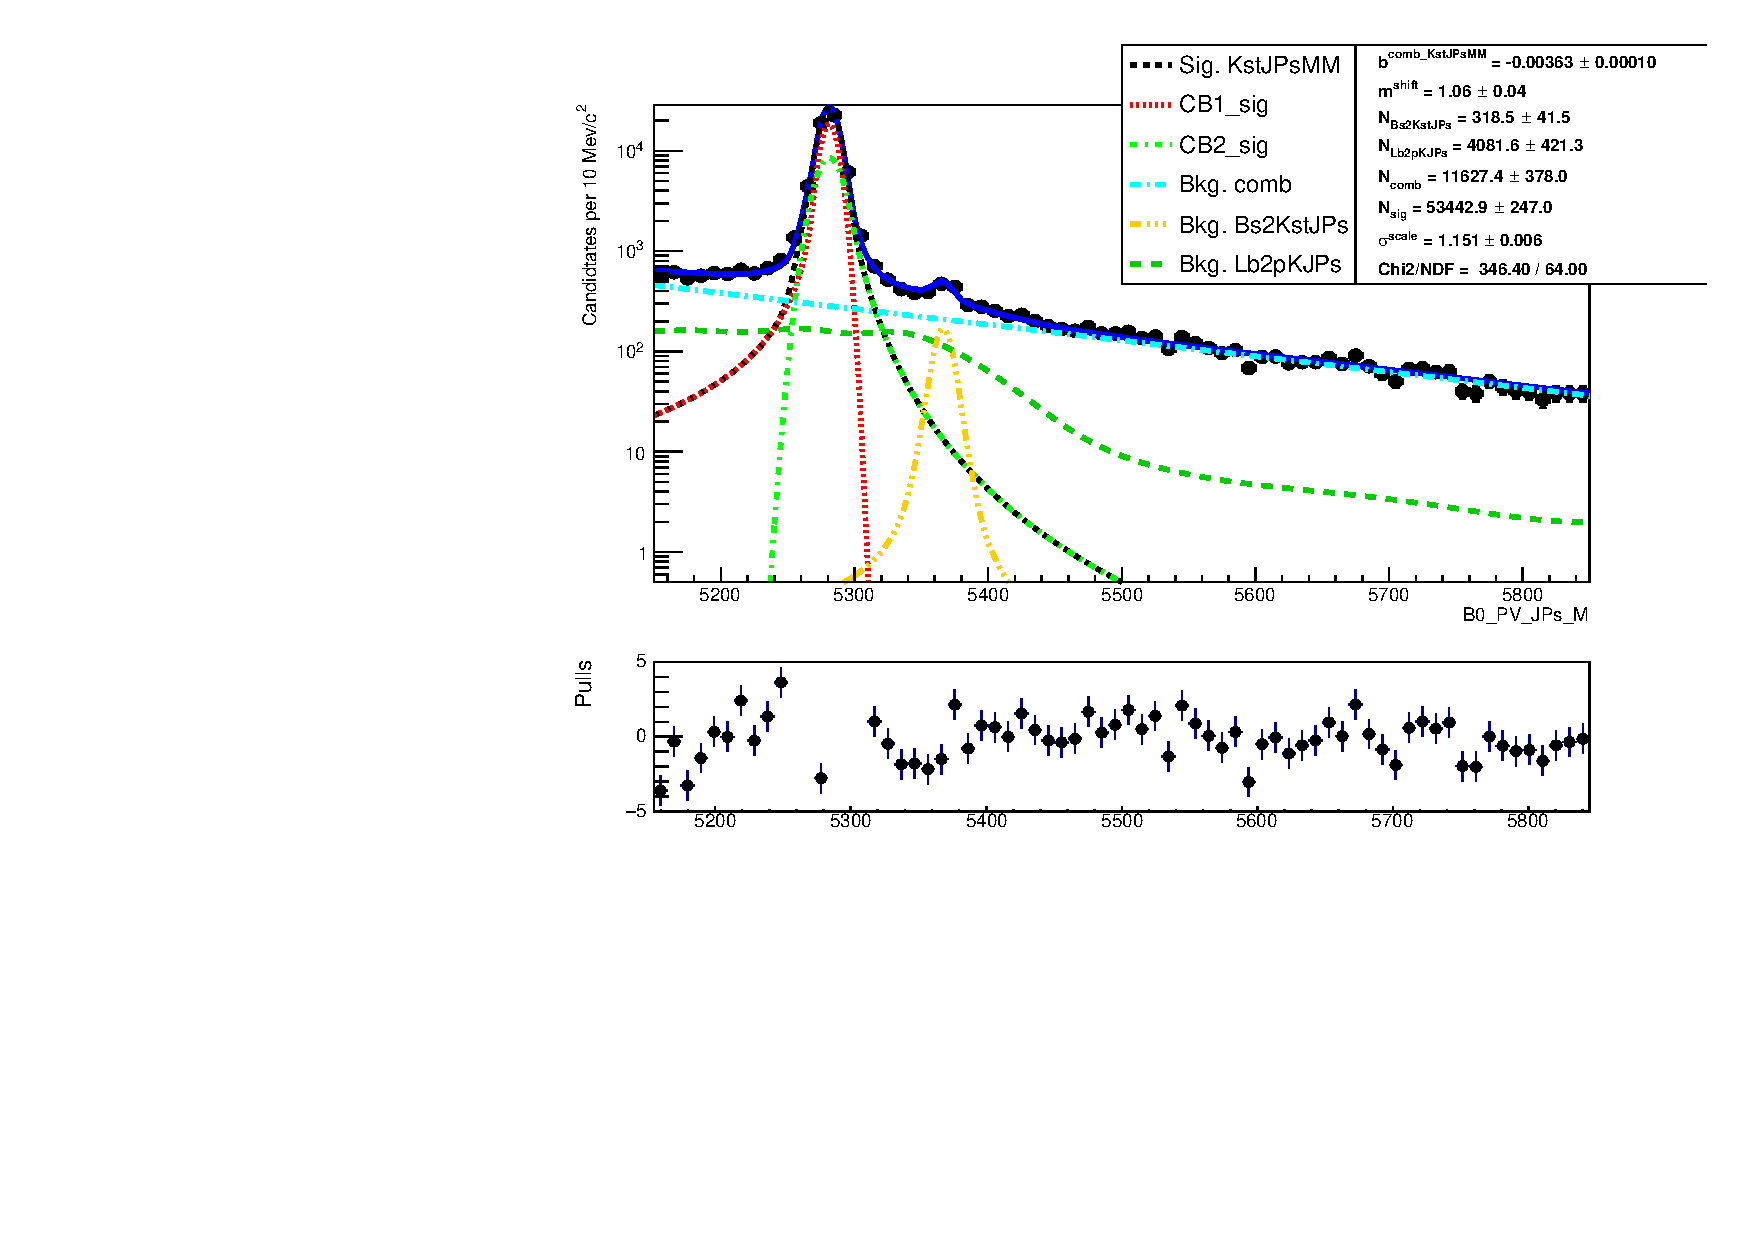
\includegraphics[width=0.7\textwidth]{RKst/figs/sW/KstJPsMM_log_fitAndRes.pdf}
\caption{Fitted 4-body invariant mass distributions of muonic resonant candidates.}
\label{fig:RKst_sW_mass}
\end{figure}

 \begin{figure}[h!]
\centering
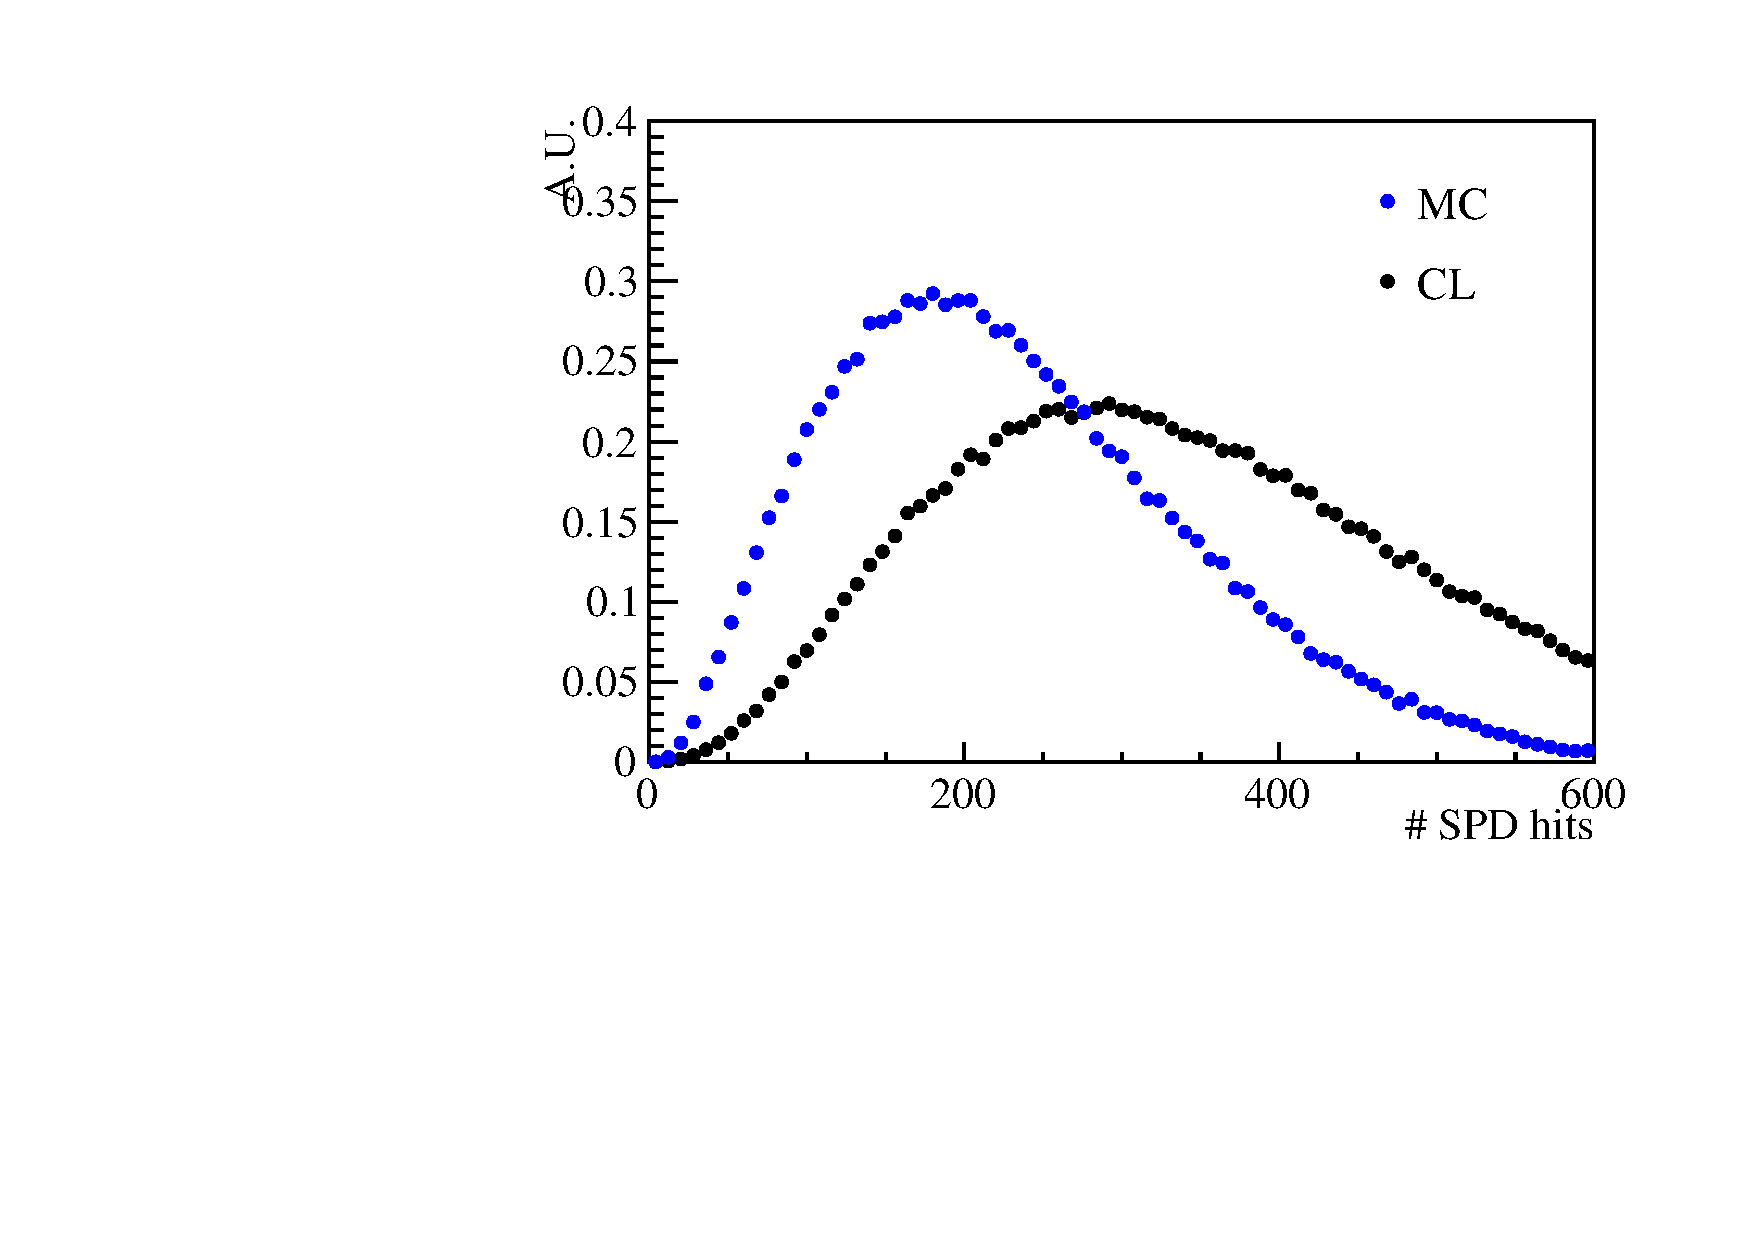
\includegraphics[width=0.48\textwidth]{RKst/figs/nspd_12.pdf}
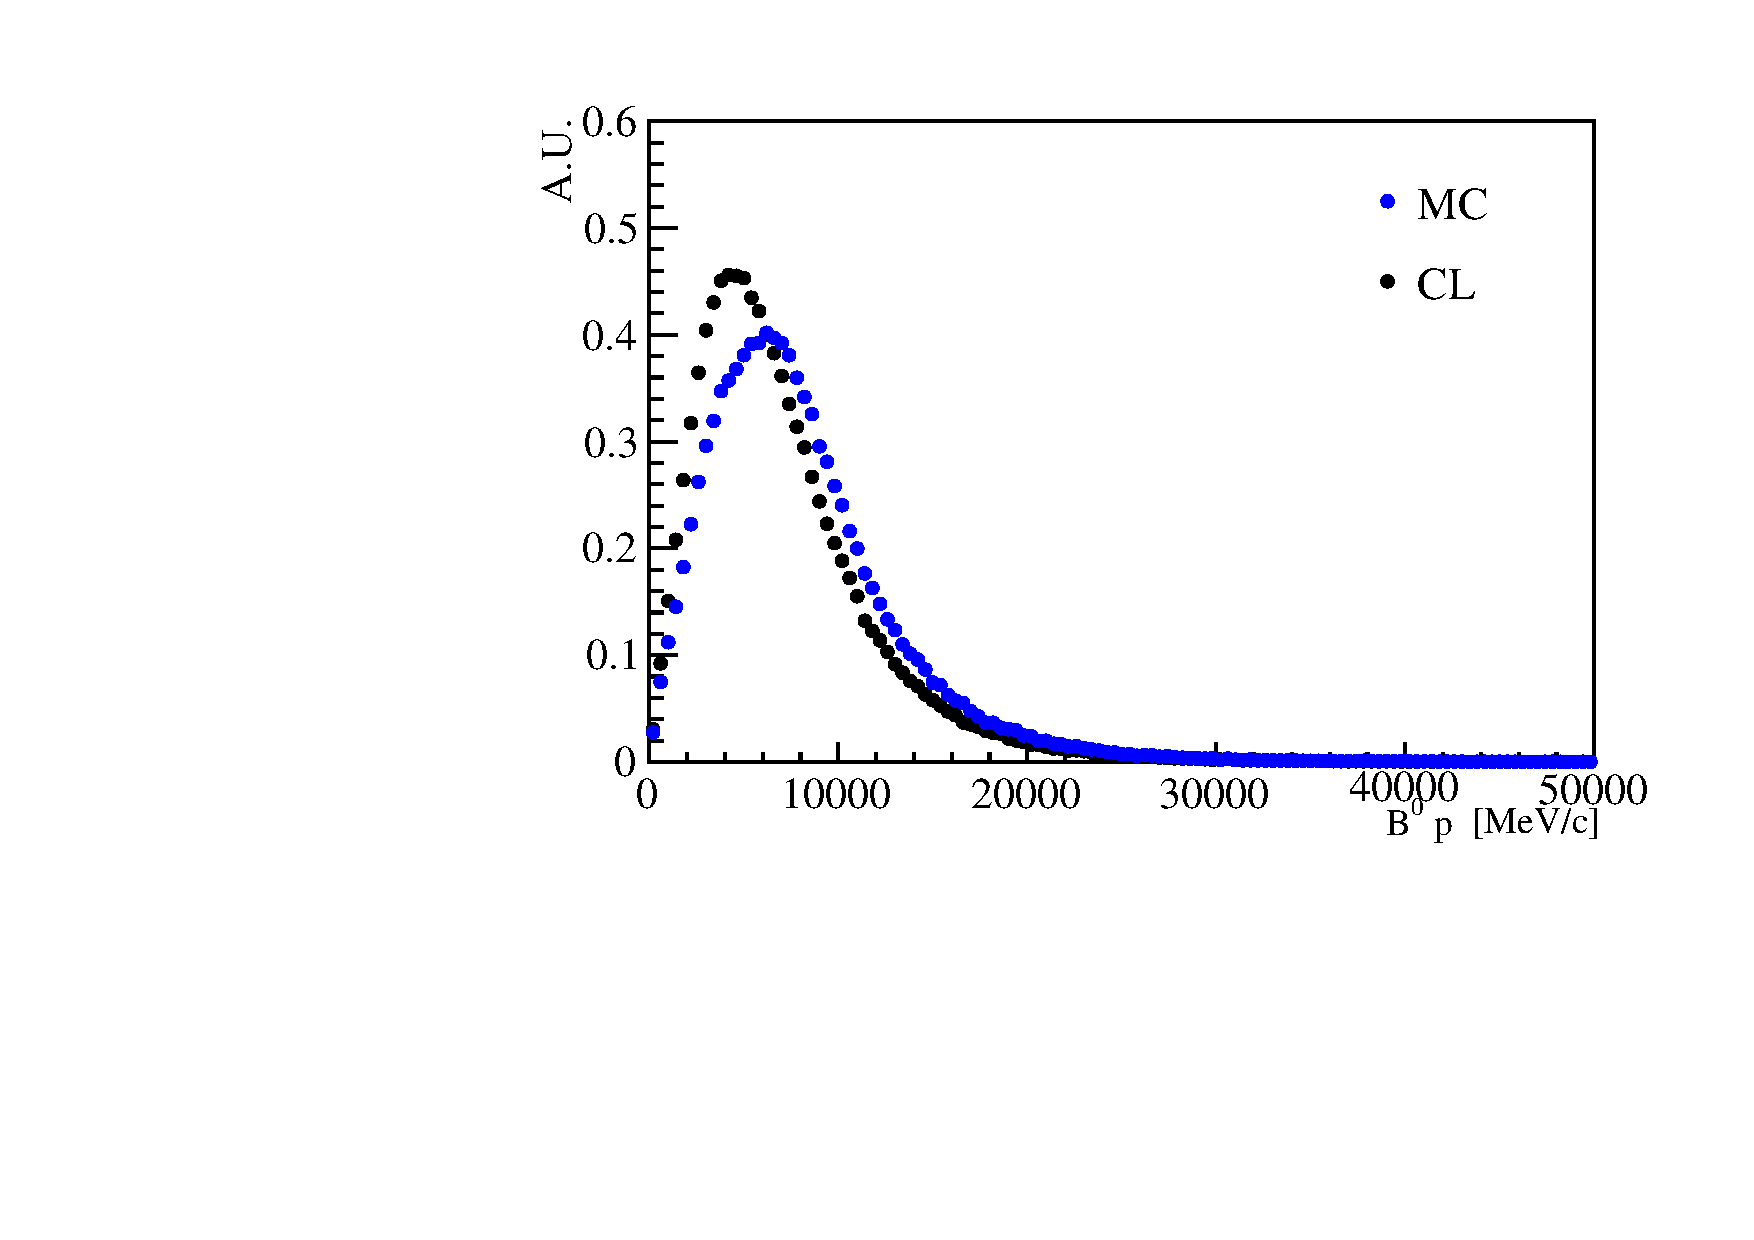
\includegraphics[width=0.48\textwidth]{RKst/figs/bpt.pdf}
\caption{Distributions of number of SPD hits (left) and \Bz transverse momentum (right) in data and MC.}
\label{fig:b0pt_nSPD_distrib}
\end{figure}

\begin{figure}[h!]
\centering
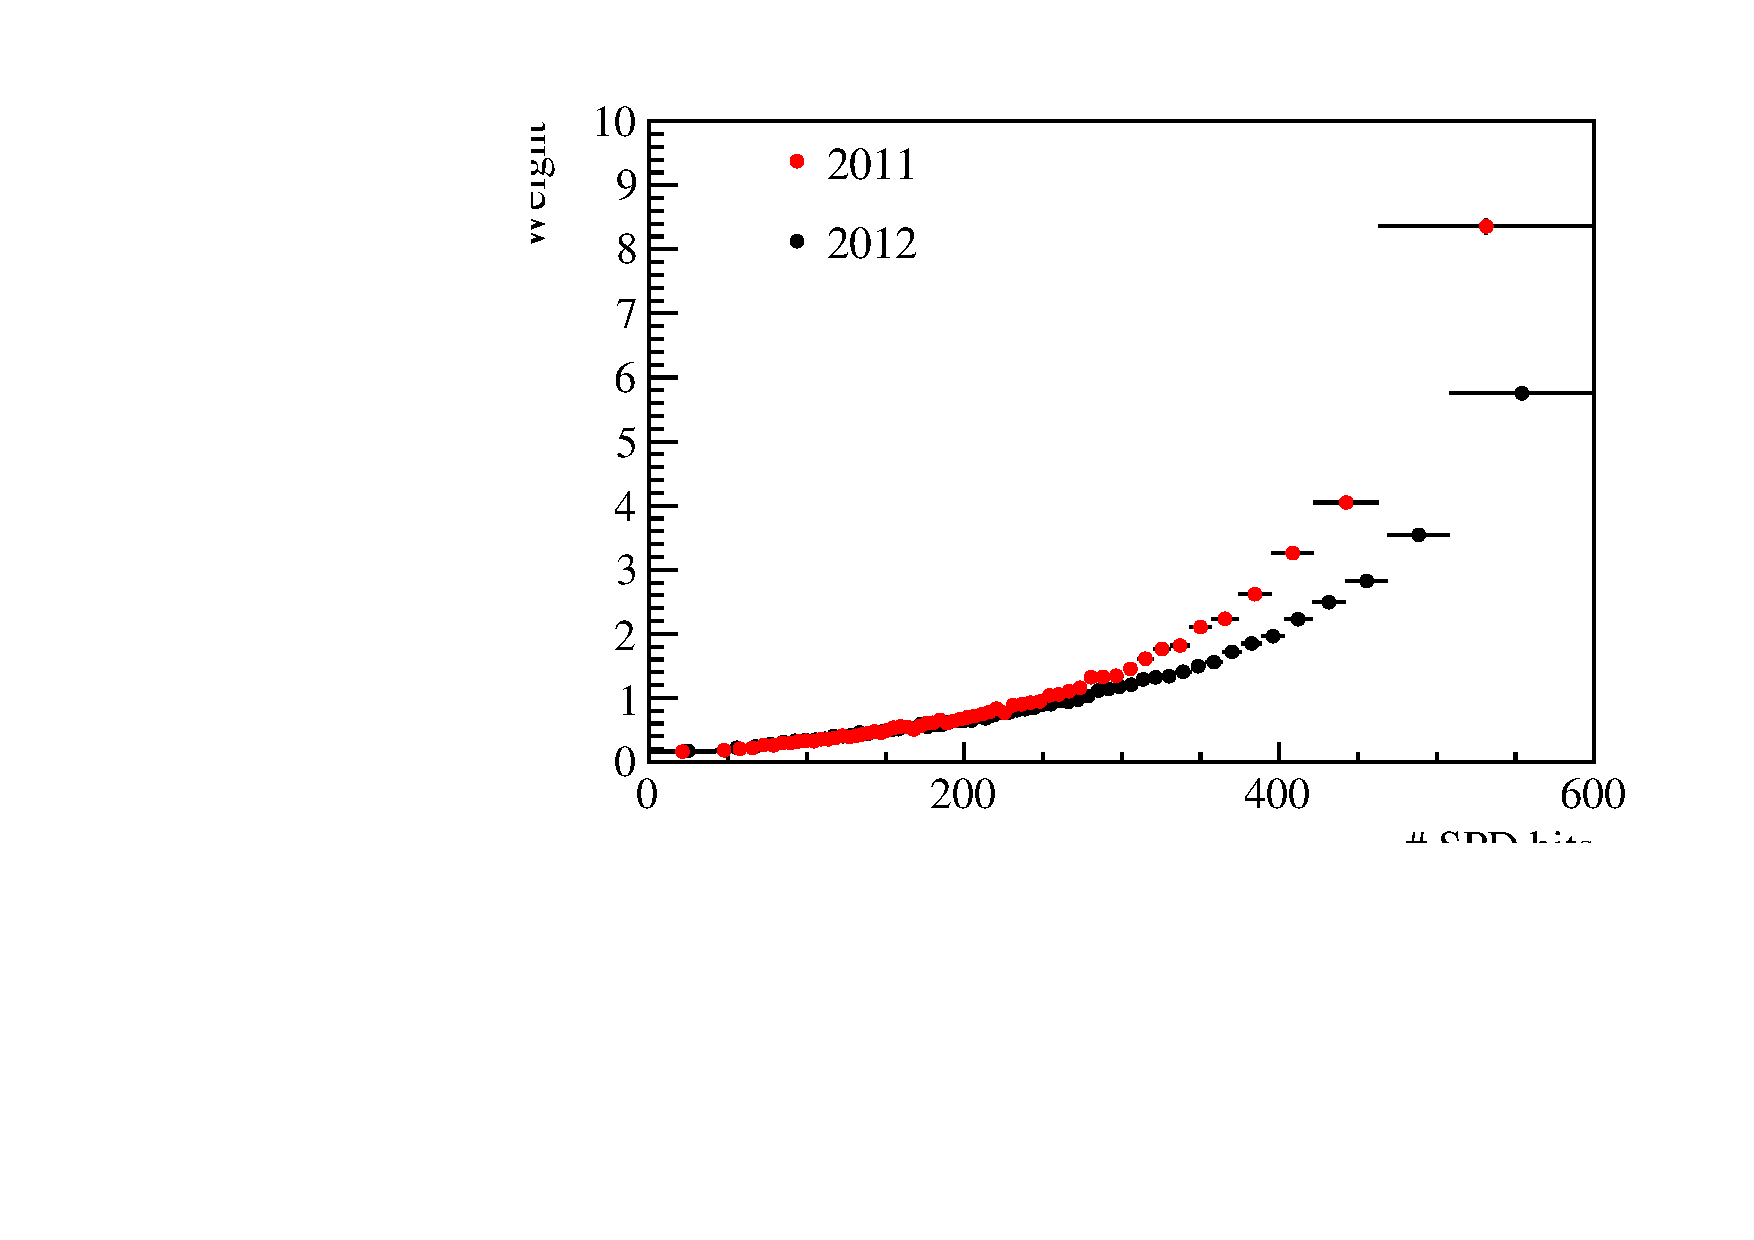
\includegraphics[width=0.48\textwidth]{RKst/figs/nspd_w.pdf}
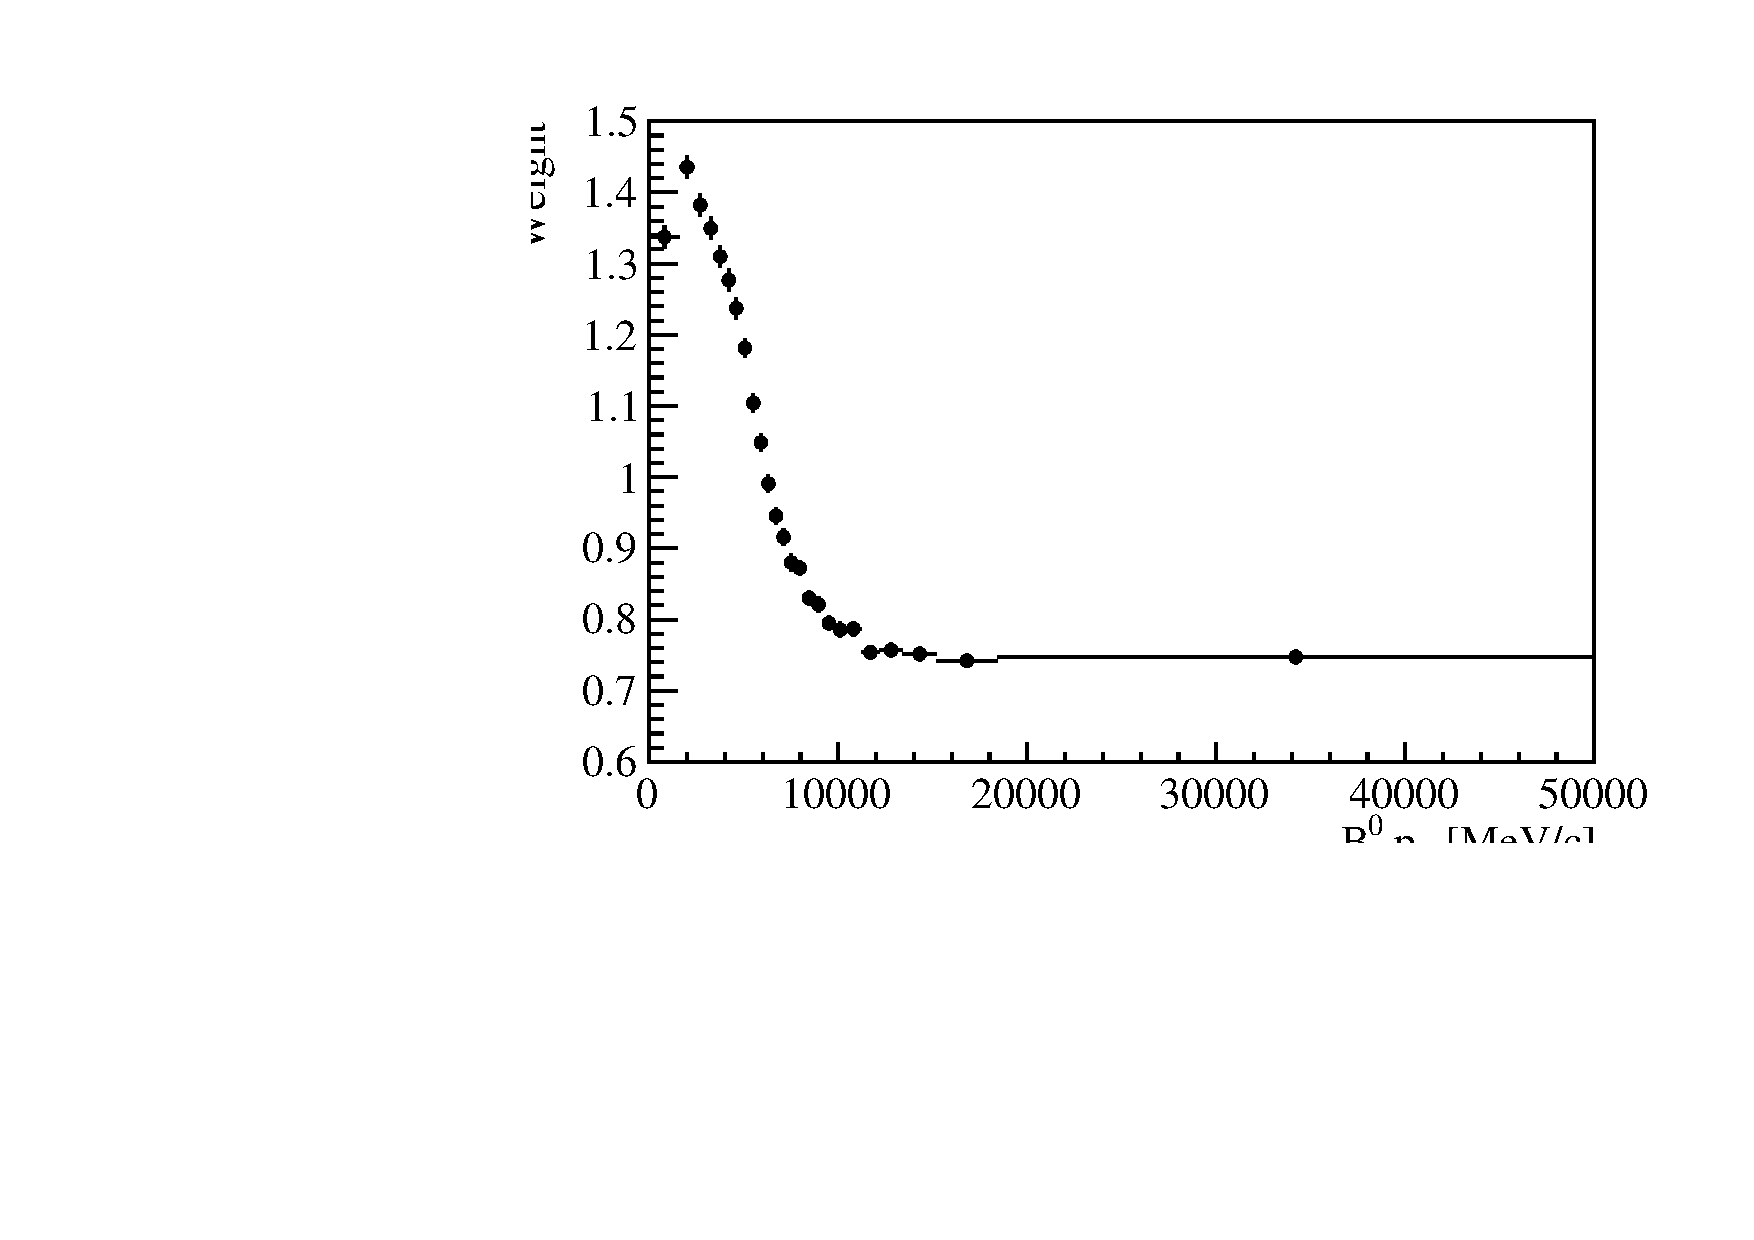
\includegraphics[width=0.48\textwidth]{RKst/figs/bpt_w.pdf}
\caption{ Ratios of simulated over real data distributions used to correct the Monte Carlo
as a function of the number of SPD hits (left) and the \Bz transverse momentum (right). }
\label{fig:b0pt_nSPD_ratios}
\end{figure}



